\chapter{The RoFI Prototypes}\label{chap:prototypes}

The RoFI project as defined in the previous chapter is broad and, therefore,
implementing all of the proposed solutions in the full depth is far beyond the
reach of the thesis. Therefore, we focused on three the most important aspects
of the RoFI project. We would like to show that:
\begin{itemize}
    \item the docking mechanism can be built and that it features claimed
    properties,
    \item integration of TCP/IP communication in the system using a custom
    hardware layer is possible; and
    \item the universal module can be built.
\end{itemize}
All the source codes and CAD models of results presented here can be found in a
Git repository \url{https://github.com/paradise-fi/RoFi}.

\section{Docking Mechanism}

\section{Inter-module Communication}

We proposed in section \ref{sec:communication} that the modules in a RoFI system
should communicate using a TCP/IP networking as it allows to easily adapt
existing algorithms and technical solutions. The proposed solution implements a
custom layer two of the standard ISO/OSI model.

To show the feasibility of the proposed solution, we have implemented a simple
prototype. The prototype does not provide any mechanical hardware, it consists
only of several interconnected development modules with microcontrollers. We
implemented a firmware for the ATMega328p microcontroller providing the dock
protocol (section \ref{sec:dock_interface}) and a corresponding part of the RoFI
driver for the ESP32 microcontroller -- dock driver, address mapping protocol
and interface for the lwIP TCP/IP stack. Both implementation can be found in the
project repository.

The ATMega328p was chosen due availability of cheap development modules in form
Arduino Nano and low-effort development. This decision allowed us to quickly get
a working prototype, however, at the cost of not providing solution with low
performance as we reached memory and computational limits of the
microcontroller. The limitations come in form of limited SPI clock speed
(100~kHz) and smaller maximal blob size (128 bytes). We consider the
implementation of the firmware straightforward and not worth further
description.

On the other hand, the implementation of the RoFI driver for ESP32 we provide is
intended for future use. The driver is written in C++14. It is structured in two
classes: \texttt{Dock} (direct interface for a single dock) and \texttt{Roif}
(network interface built on top docks).

\texttt{Dock} automatically handles communication with the docks, i.e., hides
all details of the communication (e.g., interrupt handling) and provides a
simple interface: user can supply a binary blob (in form of the \texttt{pbuf}
structure from lwIP) or be notified with an incoming blob via a callback. The
interface for changing or querying dock state (retracting or expanding of the
dock, querying the state of the power lines, etc.) is implemented in similar
fashion. Our implementation prevents congestion of the shared SPI bus by
limiting the number of pending queries per dock and therefore, allowing for fair
usage of the bus.

The challenge of the implementation was mapping SPI transaction to the interface
provided by ESP32 development framework (ESP-IDF). ESP-IDF provides a way to
queue asynchronous SPI transactions with distinct read and write phases
including delay between the phases. However, it does not support transactions
with variable length, which are required by our protocol. The transactions have
to be implemented using several SPI transaction offered by ESP-IDF. The naive
implementation is not possible as transactions from multiple docks could
interleave and therefore, yield incorrect results. There are two possible
approaches to tackle this problem: we can either queue transactions in advance
and modify them on the fly, or we can use a separate FreeRTOS task executing
blocking SPI transactions. Our implementation uses the second solution as our
analysis of the ESP-IDF source code shows that changing already queued
transactions is not safe and also, the first solution requires non-trivial
locking. The second solution also produces easier to follow code with no
explicit locking as all the locking is handled by FreeRTOS and therefore, was
chosen.

\texttt{Roif} (\emph{Ro}Fi network \emph{in}terface) provides a glue between
docks and lwIP. It handles registration of a new network interface and all the
required callbacks (as we mentioned in section \ref{sec:networking}). It also
features implementation of the address mapping protocol to determine which dock
should be used for outgoing communication.

As a by-product of the implementation of the RoFI driver, we implemented set of
C++ wrappers for the FreeRTOS API. Unlike the already existing C++ wrappers we
are aware of, we do not simply rename functions and group them in classes like
these wrappers. Our wrappers respect C++ idioms and also provide proper C++ copy
and move semantics. Such wrapper allows the user to write easier to understand
and less error-prone code. At the time of writing this theses, the FreeRTOS
wrapper was not separated into a stand-alone project.

\begin{figure}[!t]
    \centering
    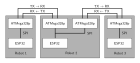
\includegraphics[width=\textwidth]{figures/communication_setup.pdf}
    \caption{The setup for our inter-module communication prototype.}
    \label{fig:comm_setup}
\end{figure}

We tested our implementation in a simple setup shown at figure
\ref{fig:comm_setup}. We used three ESP32-DevkitCs simulating module
controllers, and for Arduino Nanos simulating the docks. We wired them as shown
in the figure. Then, we were able to successfully establish both, TCP and UDP,
connections. The codes for establishing the connections are a simple example
inspired by official demo codes. There are no modification for our setup. The
example codes can be found in the project repository.

Replication of our results should be fairly straightforward as we ship all the
code as PlatformIO\footnote{\url{https://platformio.org/}} projects, therefore
no complicated toolchain setup is necessary; and also, the hardware we use is
commonly available.However, during testing of our firmware we encountered a bug
in lwIP implementation preventing a TCP connection from being opened. The bug
has been already fixed in the lwIP upstream repository, however at the time of
writing this thesis, the lwIP library shipped with ESP-IDF was not updated.
Therefore, to successfully run the TCP example, manual update of the library is
necessary.

\section{Universal Module}
